\documentclass{article}
\usepackage[backend=biber,citestyle=ieee]{biblatex}
\usepackage[english]{babel}
%\usepackage[swedish]{babel}
\usepackage{graphicx}
\usepackage{csquotes}
\usepackage{float}
\usepackage{url}
\usepackage[hidelinks]{hyperref}
\usepackage{siunitx}
\usepackage{datetime}
\usepackage[title]{appendix}
\usepackage[font={small},margin={1cm}]{caption}
\usepackage{titlesec}
\usepackage{enumitem}
\usepackage{amsmath}
\usepackage{fancyhdr}   %page header
\usepackage[margin=1in]{geometry}

\pagestyle{fancy}
\fancyhf{}

\cfoot{Page \thepage}

\usepackage[parfill]{parskip} %Line skip between paragraphs instead of indent

\usepackage{xcolor}
\usepackage{listings}   %code section 



\newcommand{\getauthor}{Eric Johansson (erjo2002@student.miun.se)\\Can Kupeli (caku2002@student.miun.se) \\Samuel Greenberg (sagr1908@student.miun.se)} %Author
\newcommand{\gettitle}{Laboration 1 \\Equations and Differencial Methods} %Title
\newcommand{\getcourse}{(MA069G, Mathematical Modelling 6hp)} %Course
\newcommand{\getsupervisor}{Cornelia Schiebold\\Magnus Eriksson\\Suprokash Hazra}


\begin{document}
  \begin{titlepage}
	\begin{center}
		\vspace*{1cm}

		
\includegraphics[width=0.8\textwidth]{imgs/msu.png}\\[0.5cm]
		\Large
		Institution of Information Systems and -Technology (IST)\\[1cm]
		\Huge
		\rule{\textwidth}{1px}
		\textbf{\gettitle}
		\rule[0.5cm]{\textwidth}{1px}

		\large
		\getcourse{}
		\vspace{1cm}

        \Large
		\textbf{\getauthor}\\

		\vfill


		\vspace{0.8cm}

		\small
		\today \\
		\Large
		\textbf{Supervisor:}\\
		\getsupervisor{}

	\end{center}
\end{titlepage}
\tableofcontents
\newpage

  
\section{}

\begin{figure}[h]
	\centering
	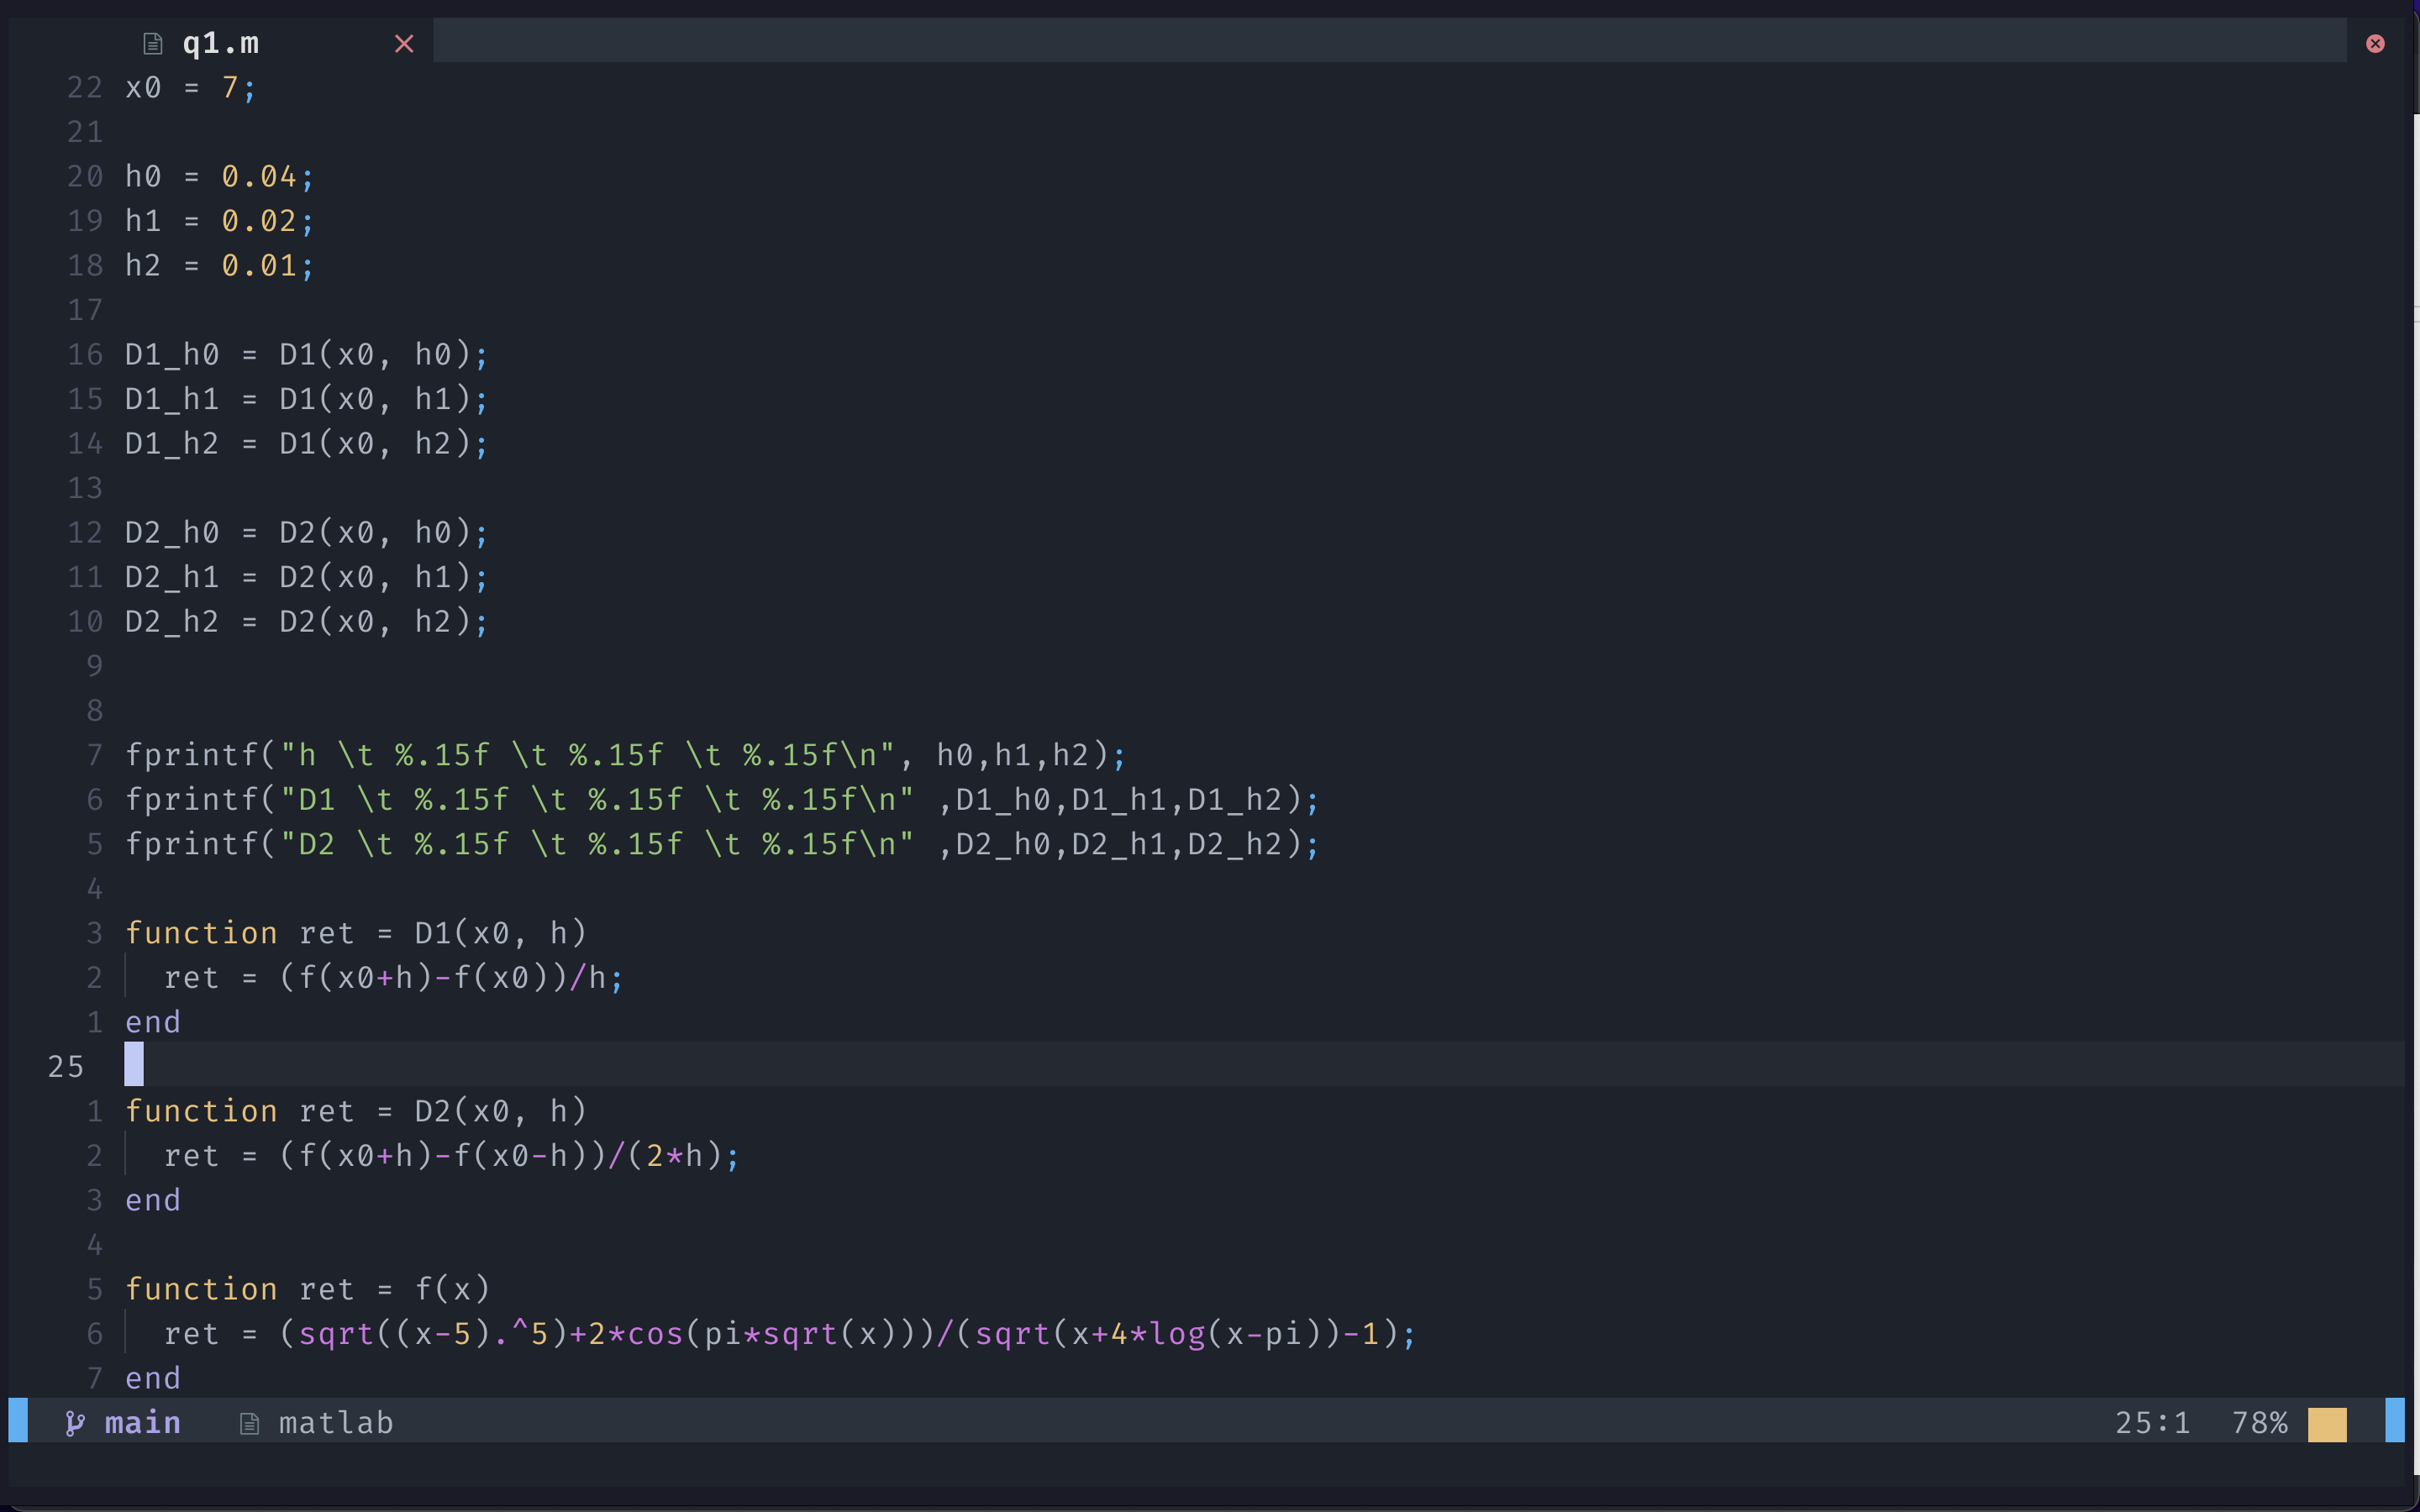
\includegraphics[width=\textwidth]{imgs/q1_code.png}
	\caption{Code for question one}
	\label{fig:q1_code}
\end{figure}

\begin{figure}[h]
	\centering
	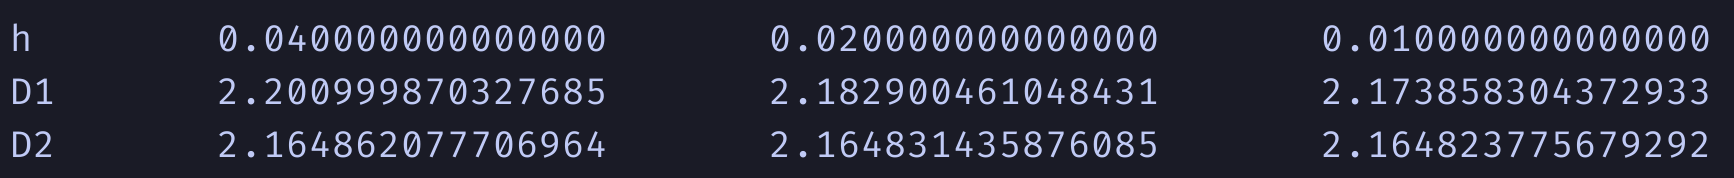
\includegraphics[width=\textwidth]{imgs/q1_results.png}
	\caption{Output for question one}
	\label{fig:q1_results}
\end{figure}

By these results we can deduce that D2, the central difference, is closer to the actual value of $f^\prime(x_0)$. This is because the method has a
truncation error of $O(h^2)$ whereas the forward difference only has $O(h)$. $O(h^{2})$ is more prefferable to $O(h)$ because when $\lim_{h \to 0}$ the term $O(h^{2})$ converges towards $0$ faster than $O(h)$.

\newpage
\section{}
\begin{figure}[H]
	\centering
	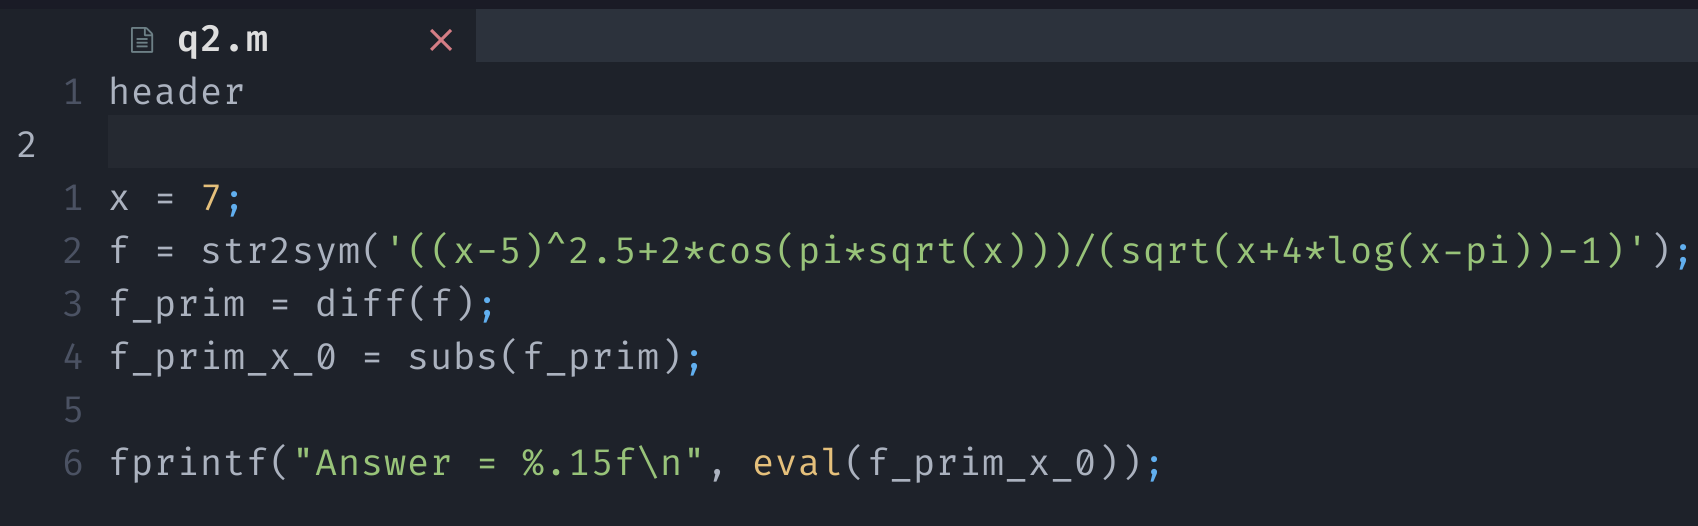
\includegraphics[width=\textwidth{}]{imgs/q2_code.png}
	\caption{Code for question 2}
	\label{fig:q2_code}
\end{figure}

\begin{figure}[H]
	\centering
	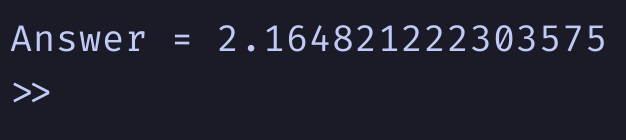
\includegraphics[width=0.5\textwidth]{imgs/q2_results.png}
	\caption{Results for question 2}
	\label{fig:q2_results}
\end{figure}

We can see here that the answer we got is the same as the real value up to 15 decimal places.

\newpage
\section{}
\begin{figure}[H]
	\centering
	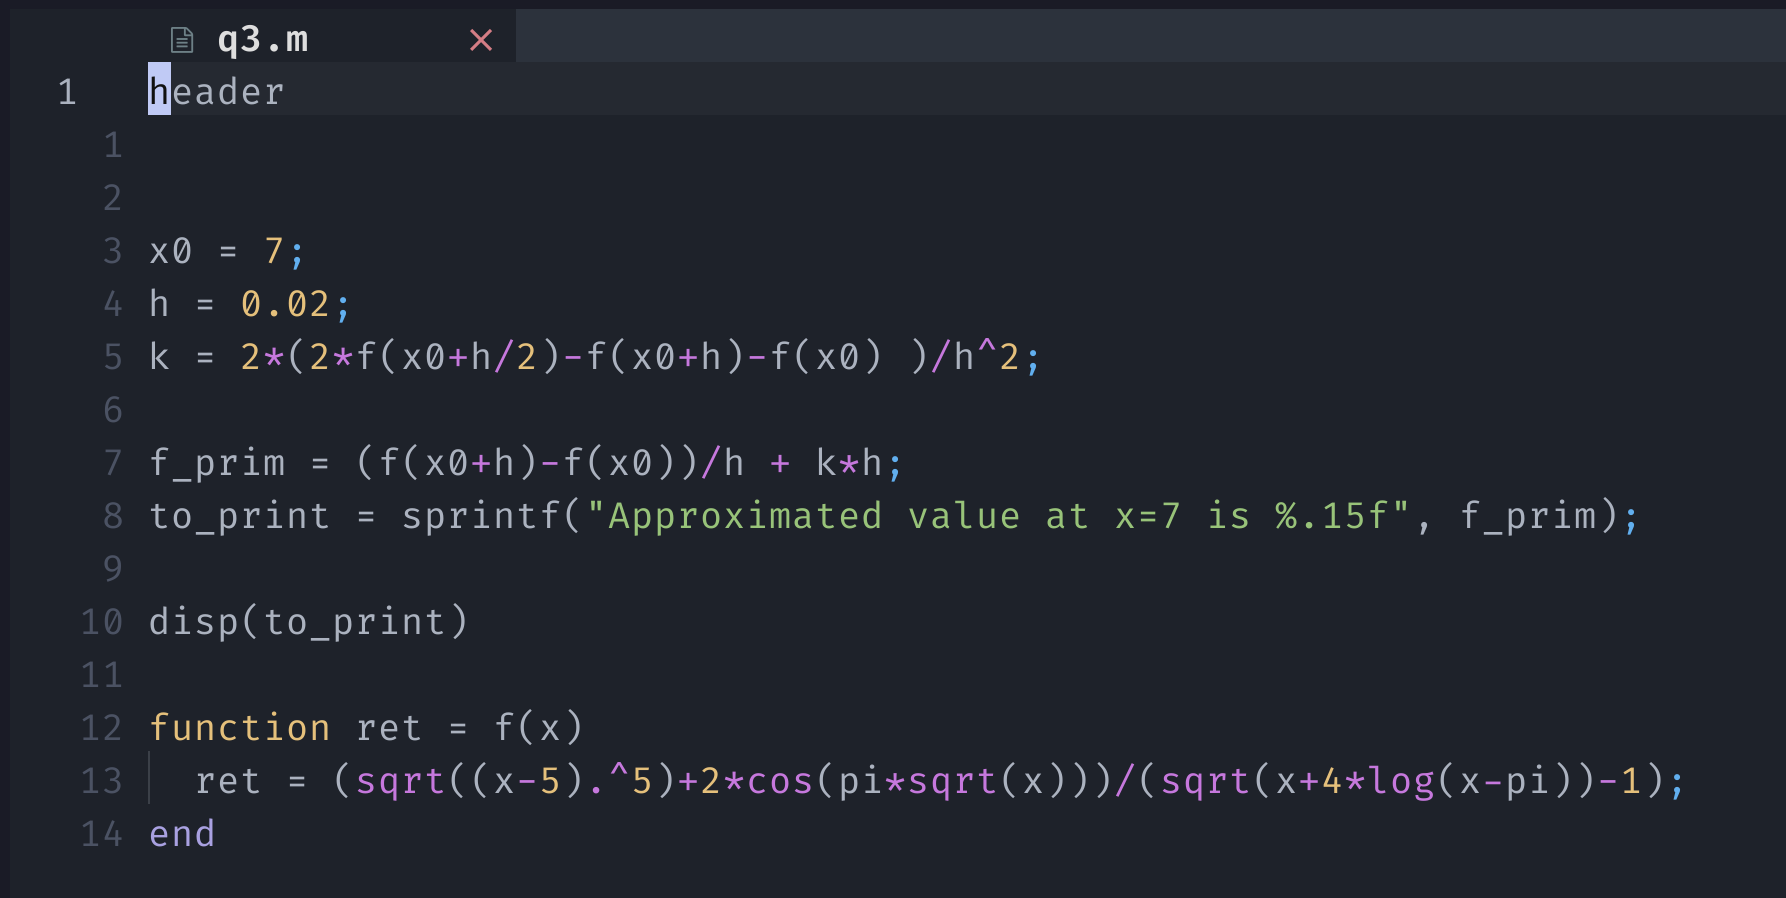
\includegraphics[width=0.8\textwidth]{imgs/q3_code.png}
	\caption{Code for question 3}
	\label{fig:q3_code}
\end{figure}

\begin{figure}[H]
	\centering
	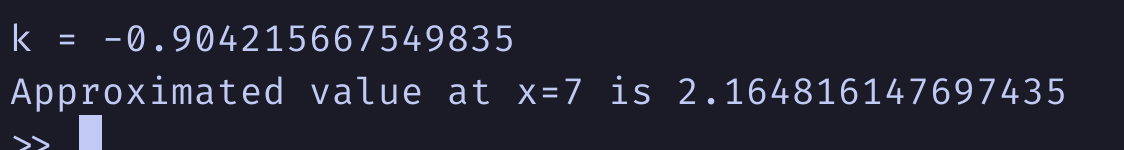
\includegraphics[width=0.8\textwidth]{imgs/q3_results.png}
	\caption{Results for question 3}
	\label{fig:q3_result}
\end{figure}

The answer is not exact because our $h$-value is not close enough to $0$ which means that our approximation of $k$ won't be exact.


\newpage
\section{}
\begin{figure}[H]
	\centering
	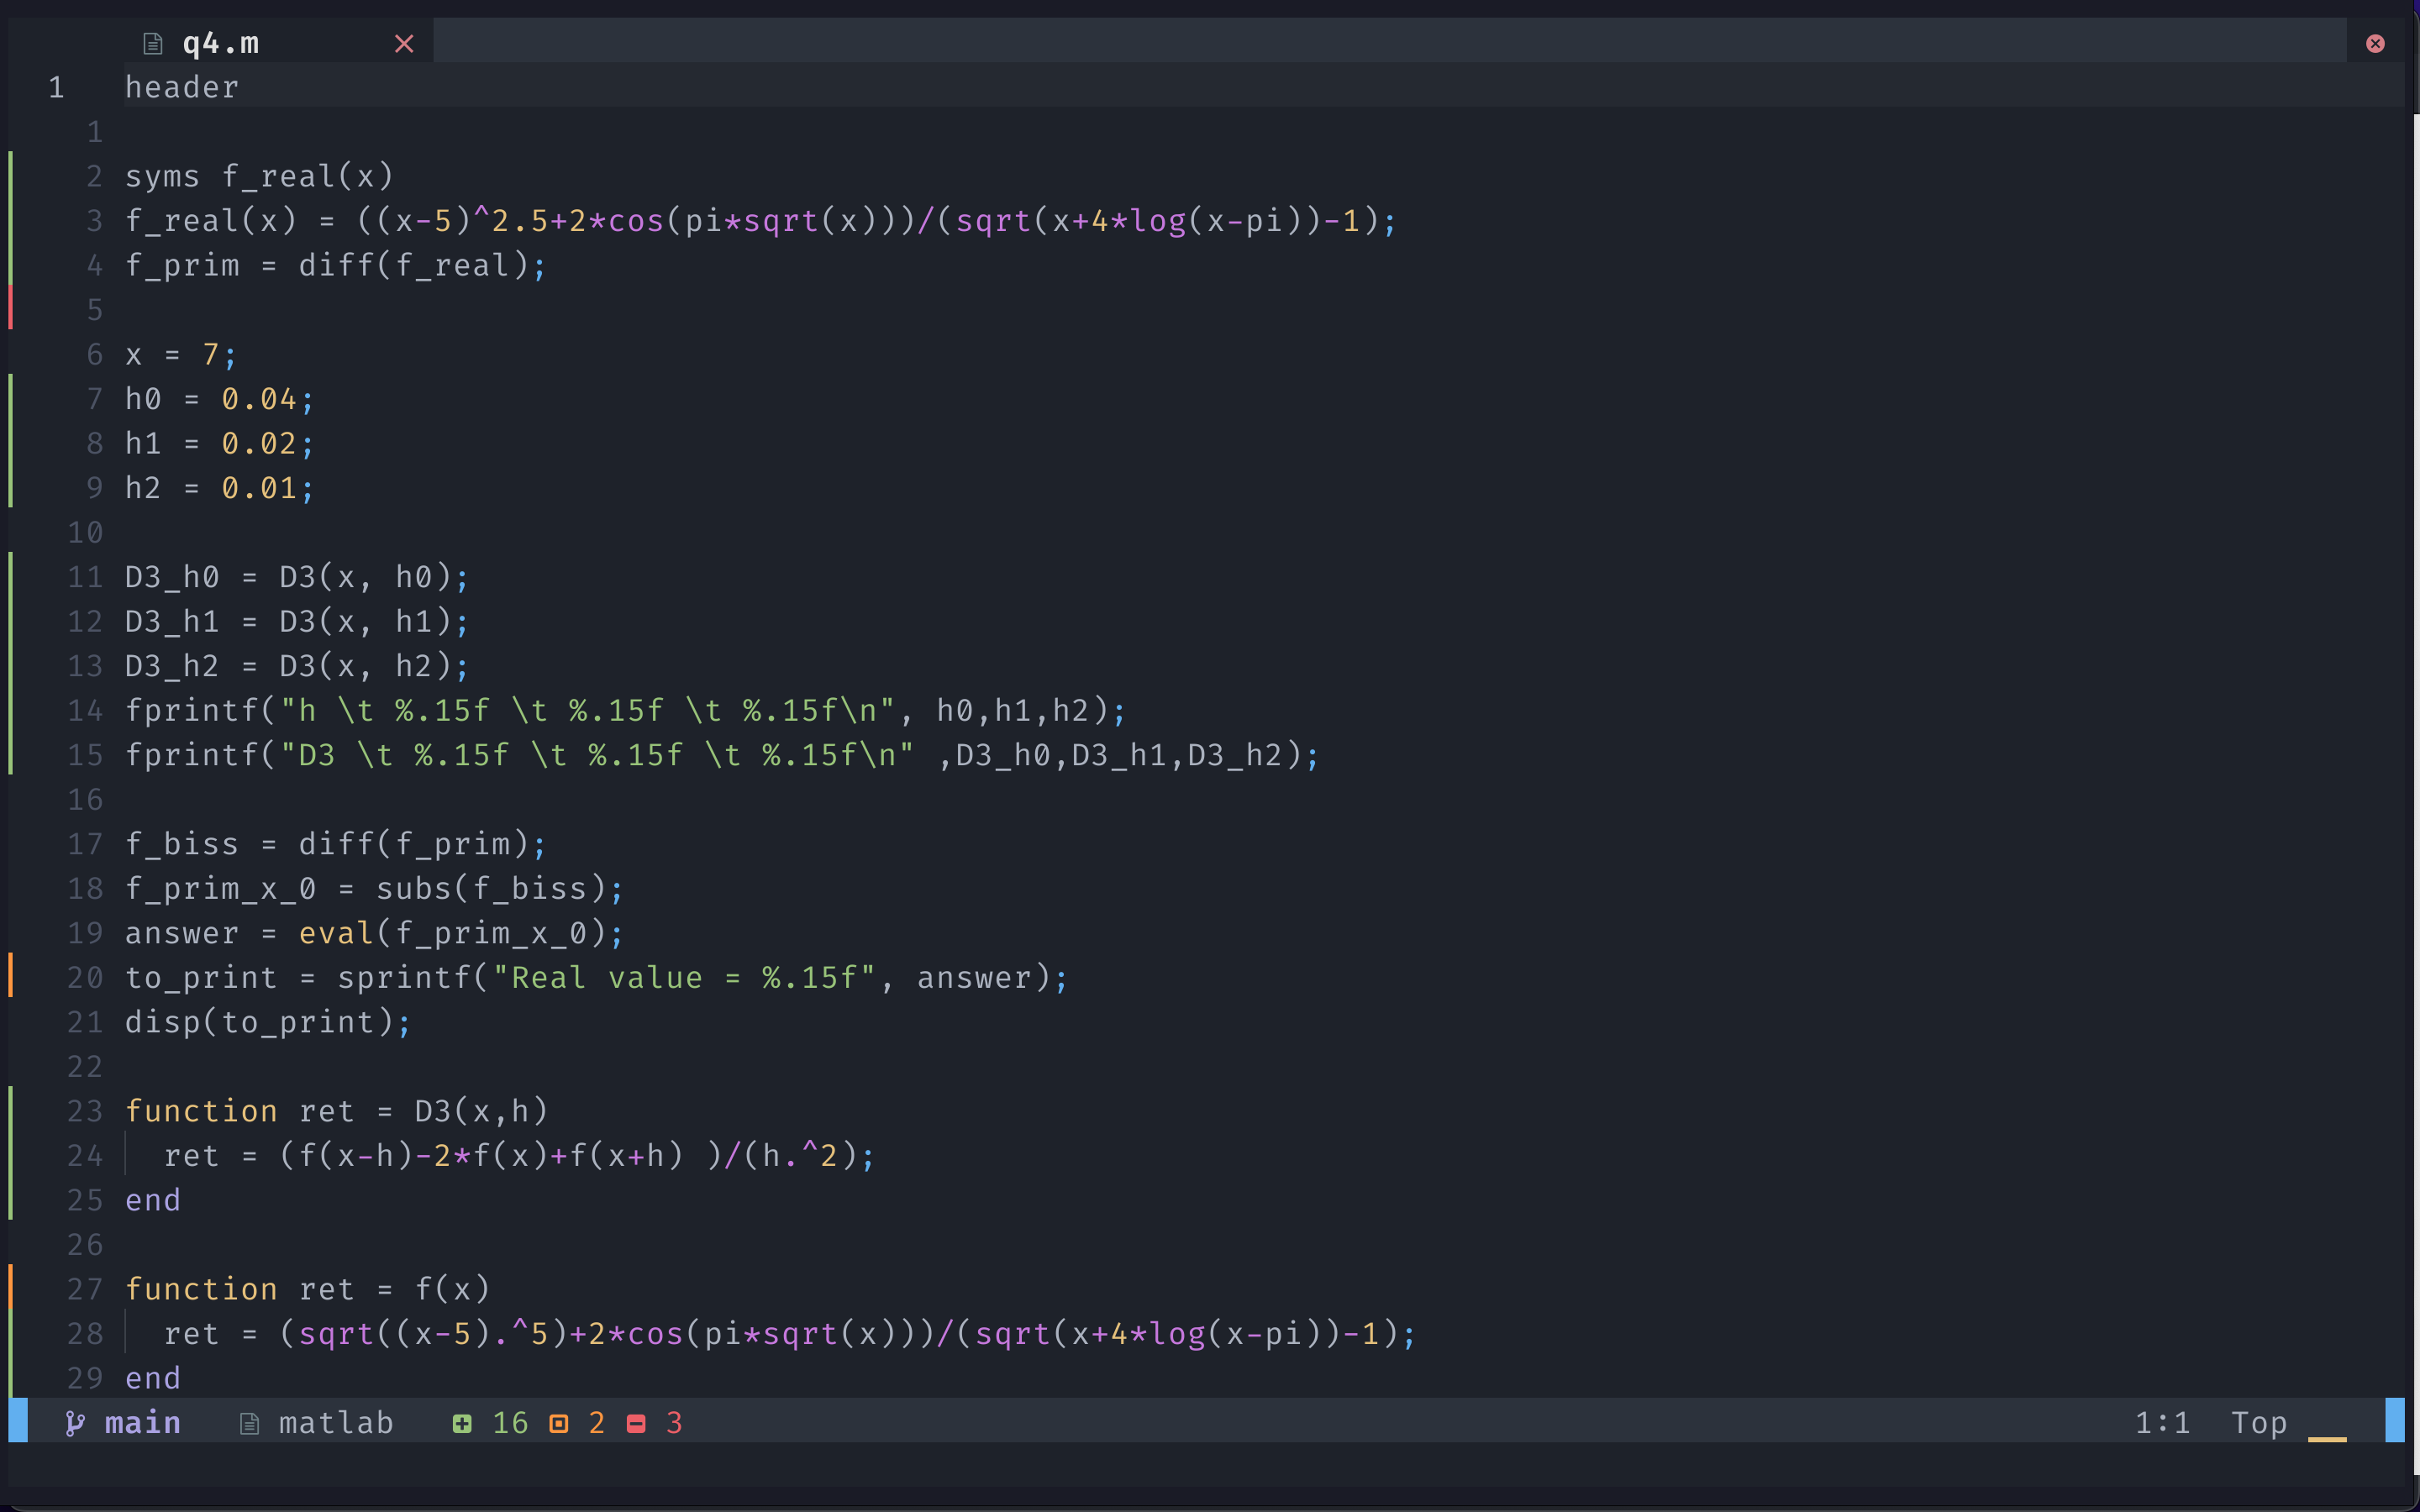
\includegraphics[width=\textwidth]{imgs/q4_code.png}
	\caption{Code for question 4}
	\label{fig:q4_code}
\end{figure}

\begin{figure}[H]
	\centering
	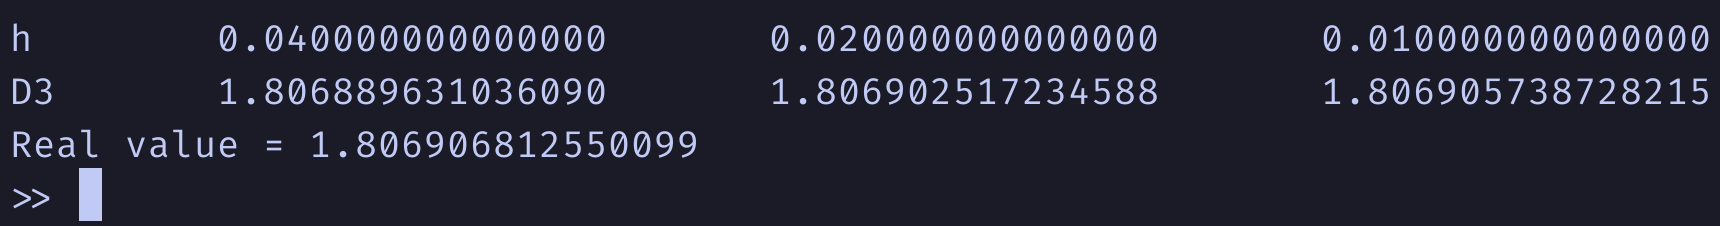
\includegraphics[width=\textwidth]{imgs/q4_results.png}
	\caption{Results for question 4}
	\label{fig:q4_result}
\end{figure}

\newpage
\section{}

\begin{figure}[H]
	\centering
	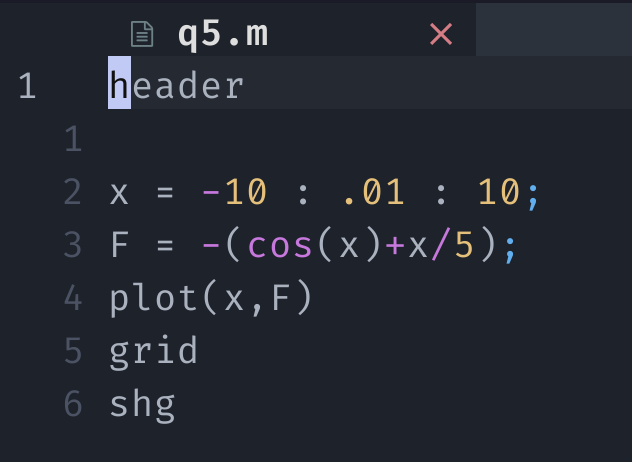
\includegraphics[width=0.5\textwidth]{imgs/q5_code.png}
	\caption{Code for question 5}
	\label{fig:q5_code}
\end{figure}

\begin{figure}[H]
	\centering
	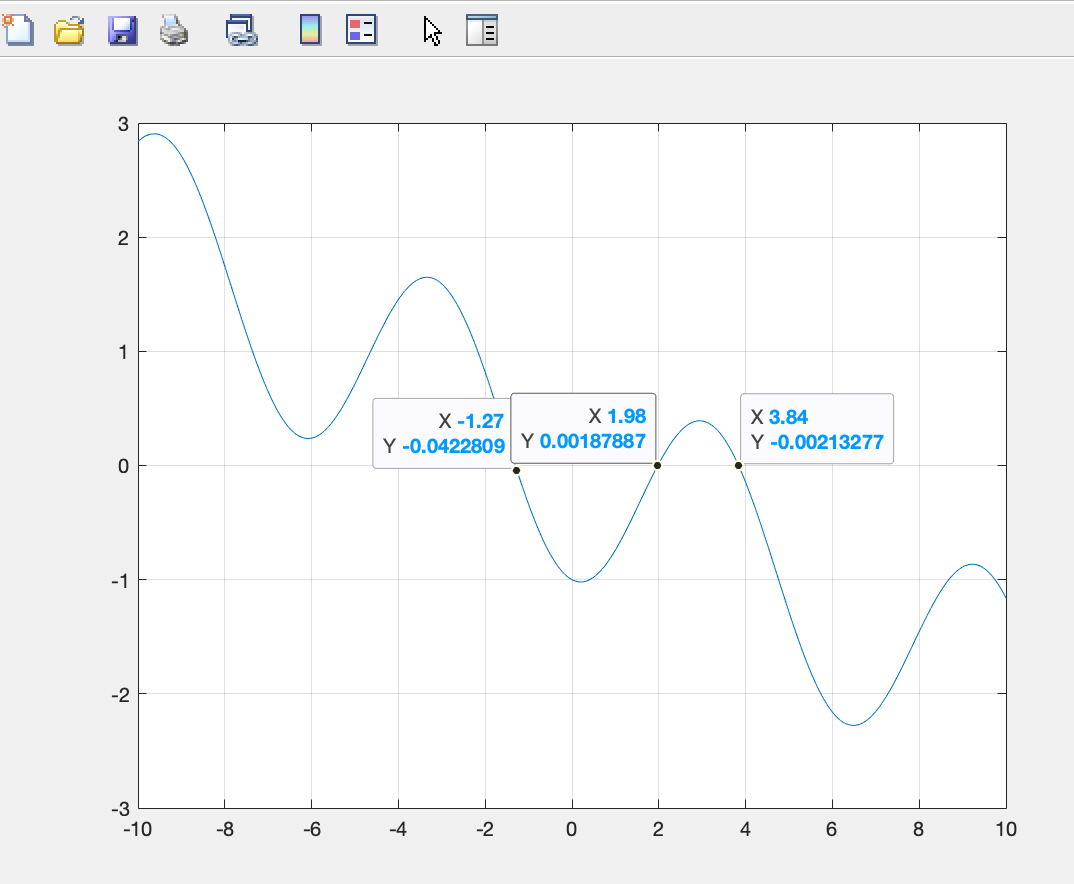
\includegraphics[width=0.8\textwidth]{imgs/q5_results.png}
	\caption{Results for question 5}
	\label{fig:q5_result}
\end{figure}

\newpage
\section{}
\begin{figure}[H]
	\centering
	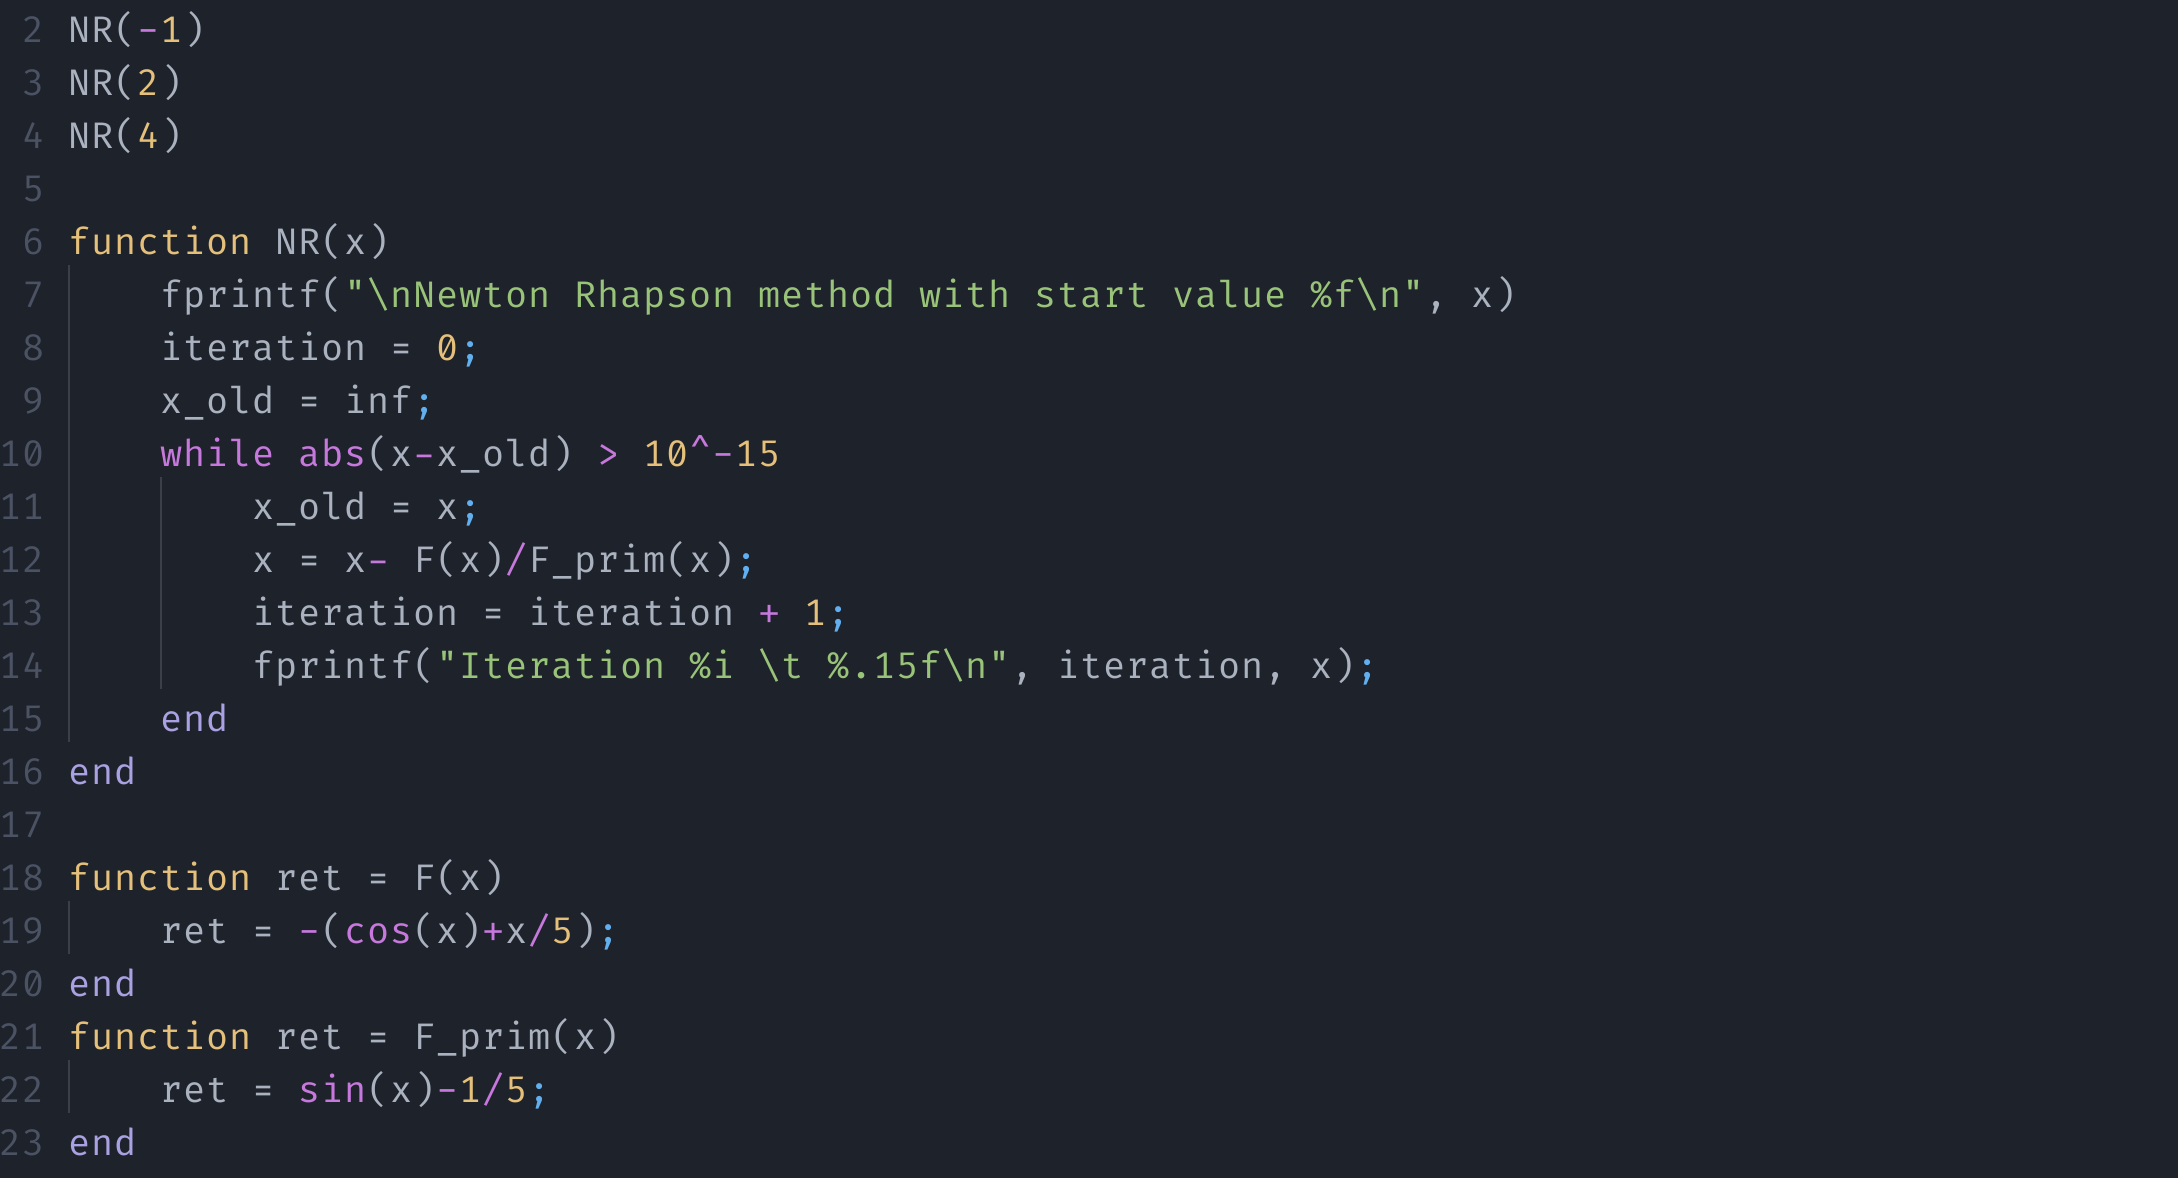
\includegraphics[width=0.8\textwidth]{imgs/q6_code.png}
	\caption{Code for question 6}
	\label{fig:q6_code}
\end{figure}

\begin{figure}[H]
	\centering
	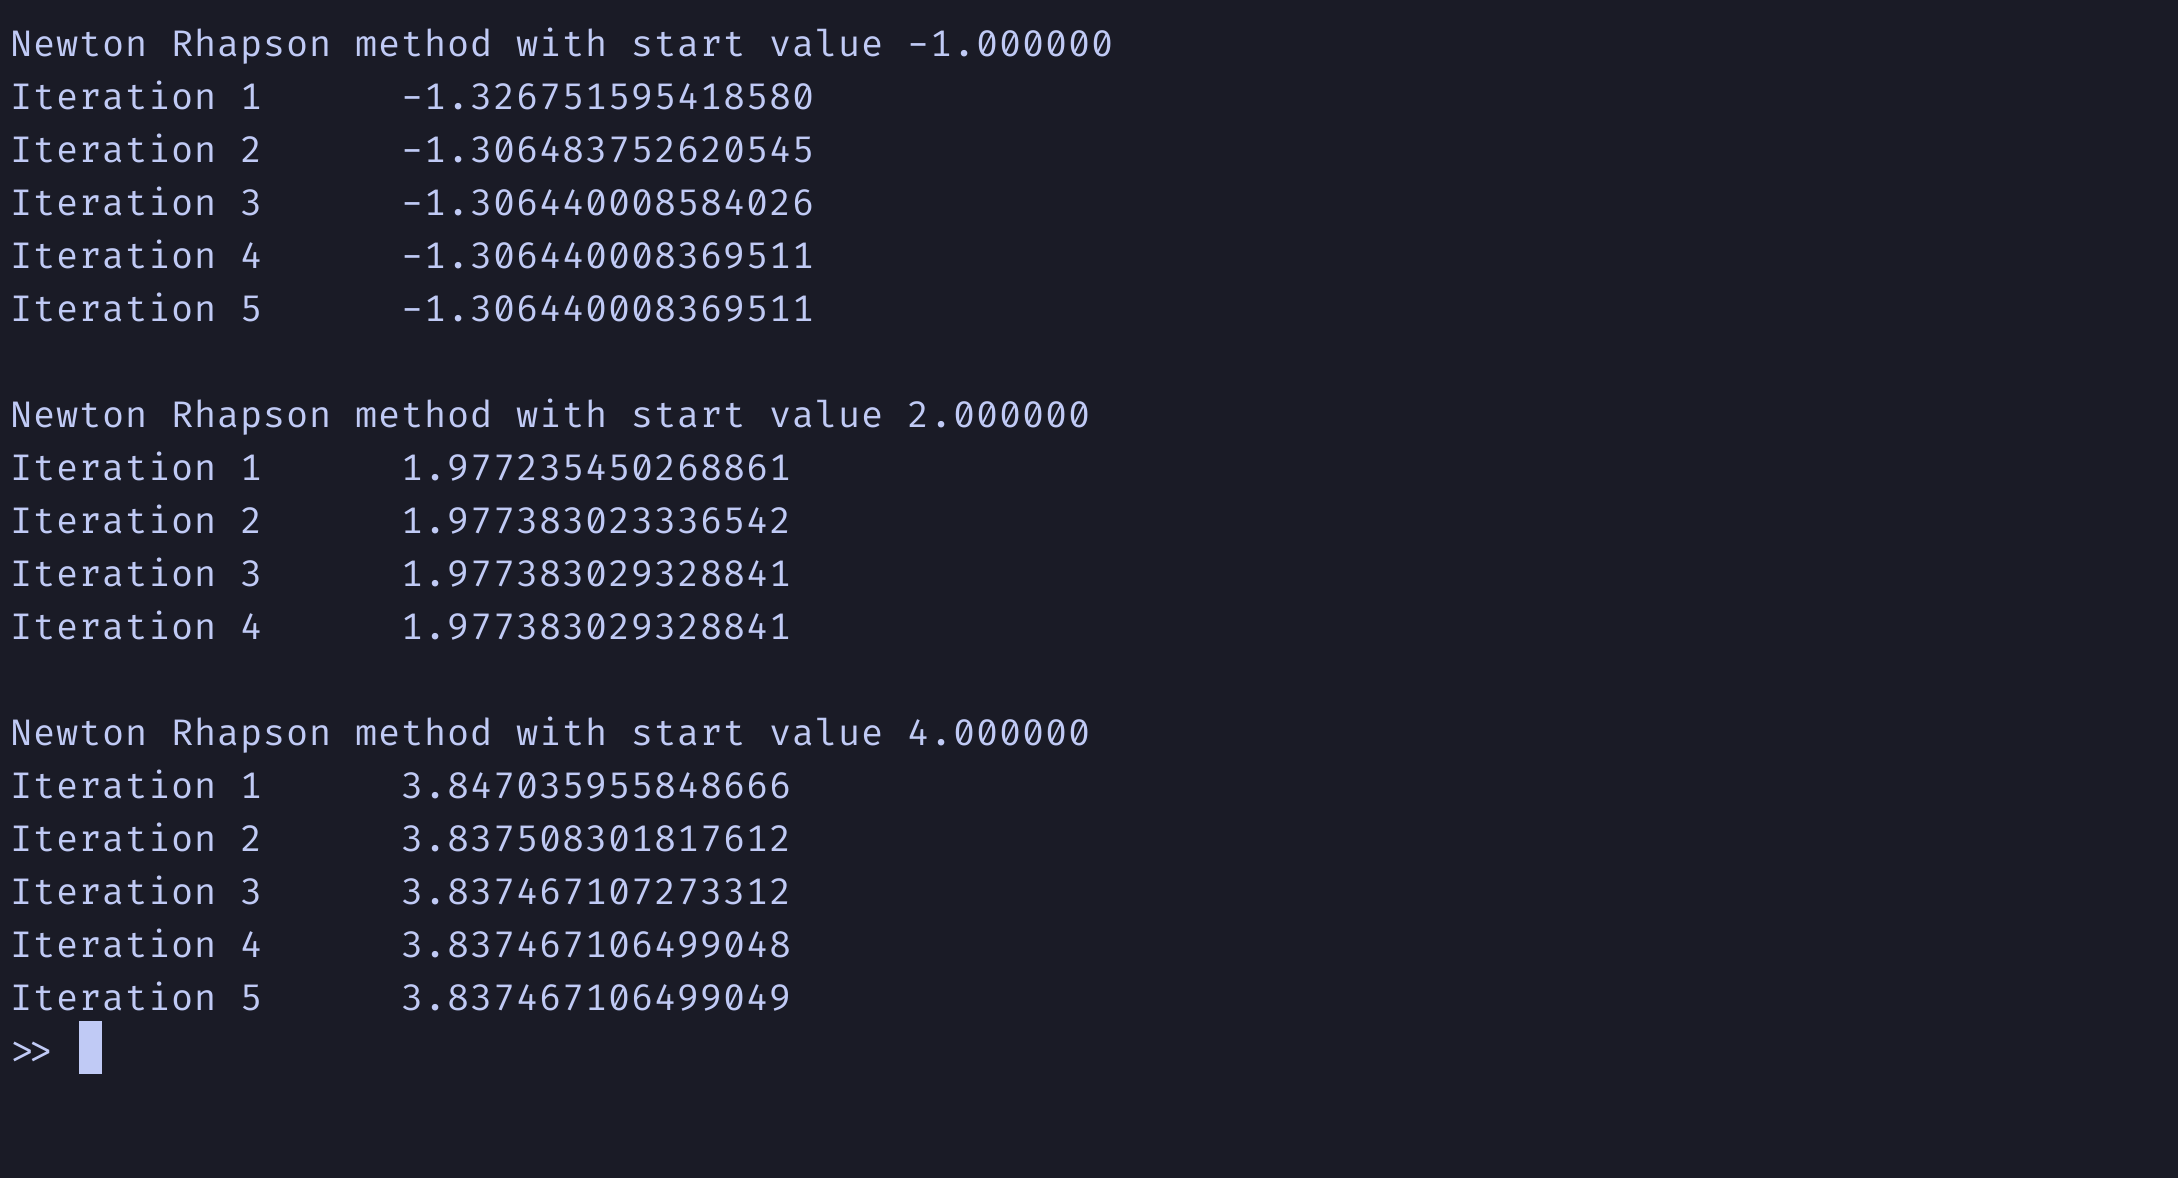
\includegraphics[width=0.8\textwidth]{imgs/q6_results.png}
	\caption{Results for question 6}
	\label{fig:q6_result}
\end{figure}

If we chose a starting value of 3 we could see that the script did not converge so it kept repeating forever. The Newton Rhapson method does not converge if the derivative is $0$ at the chosen starting point.

We can see that even with a small tolerance of $10^{-15}$ we only need around $4-5$ iterations to reach a root. We also tried with other tolerances but showing each result would take up too much space.

\newpage
\section{}
\begin{figure}[H]
	\centering
	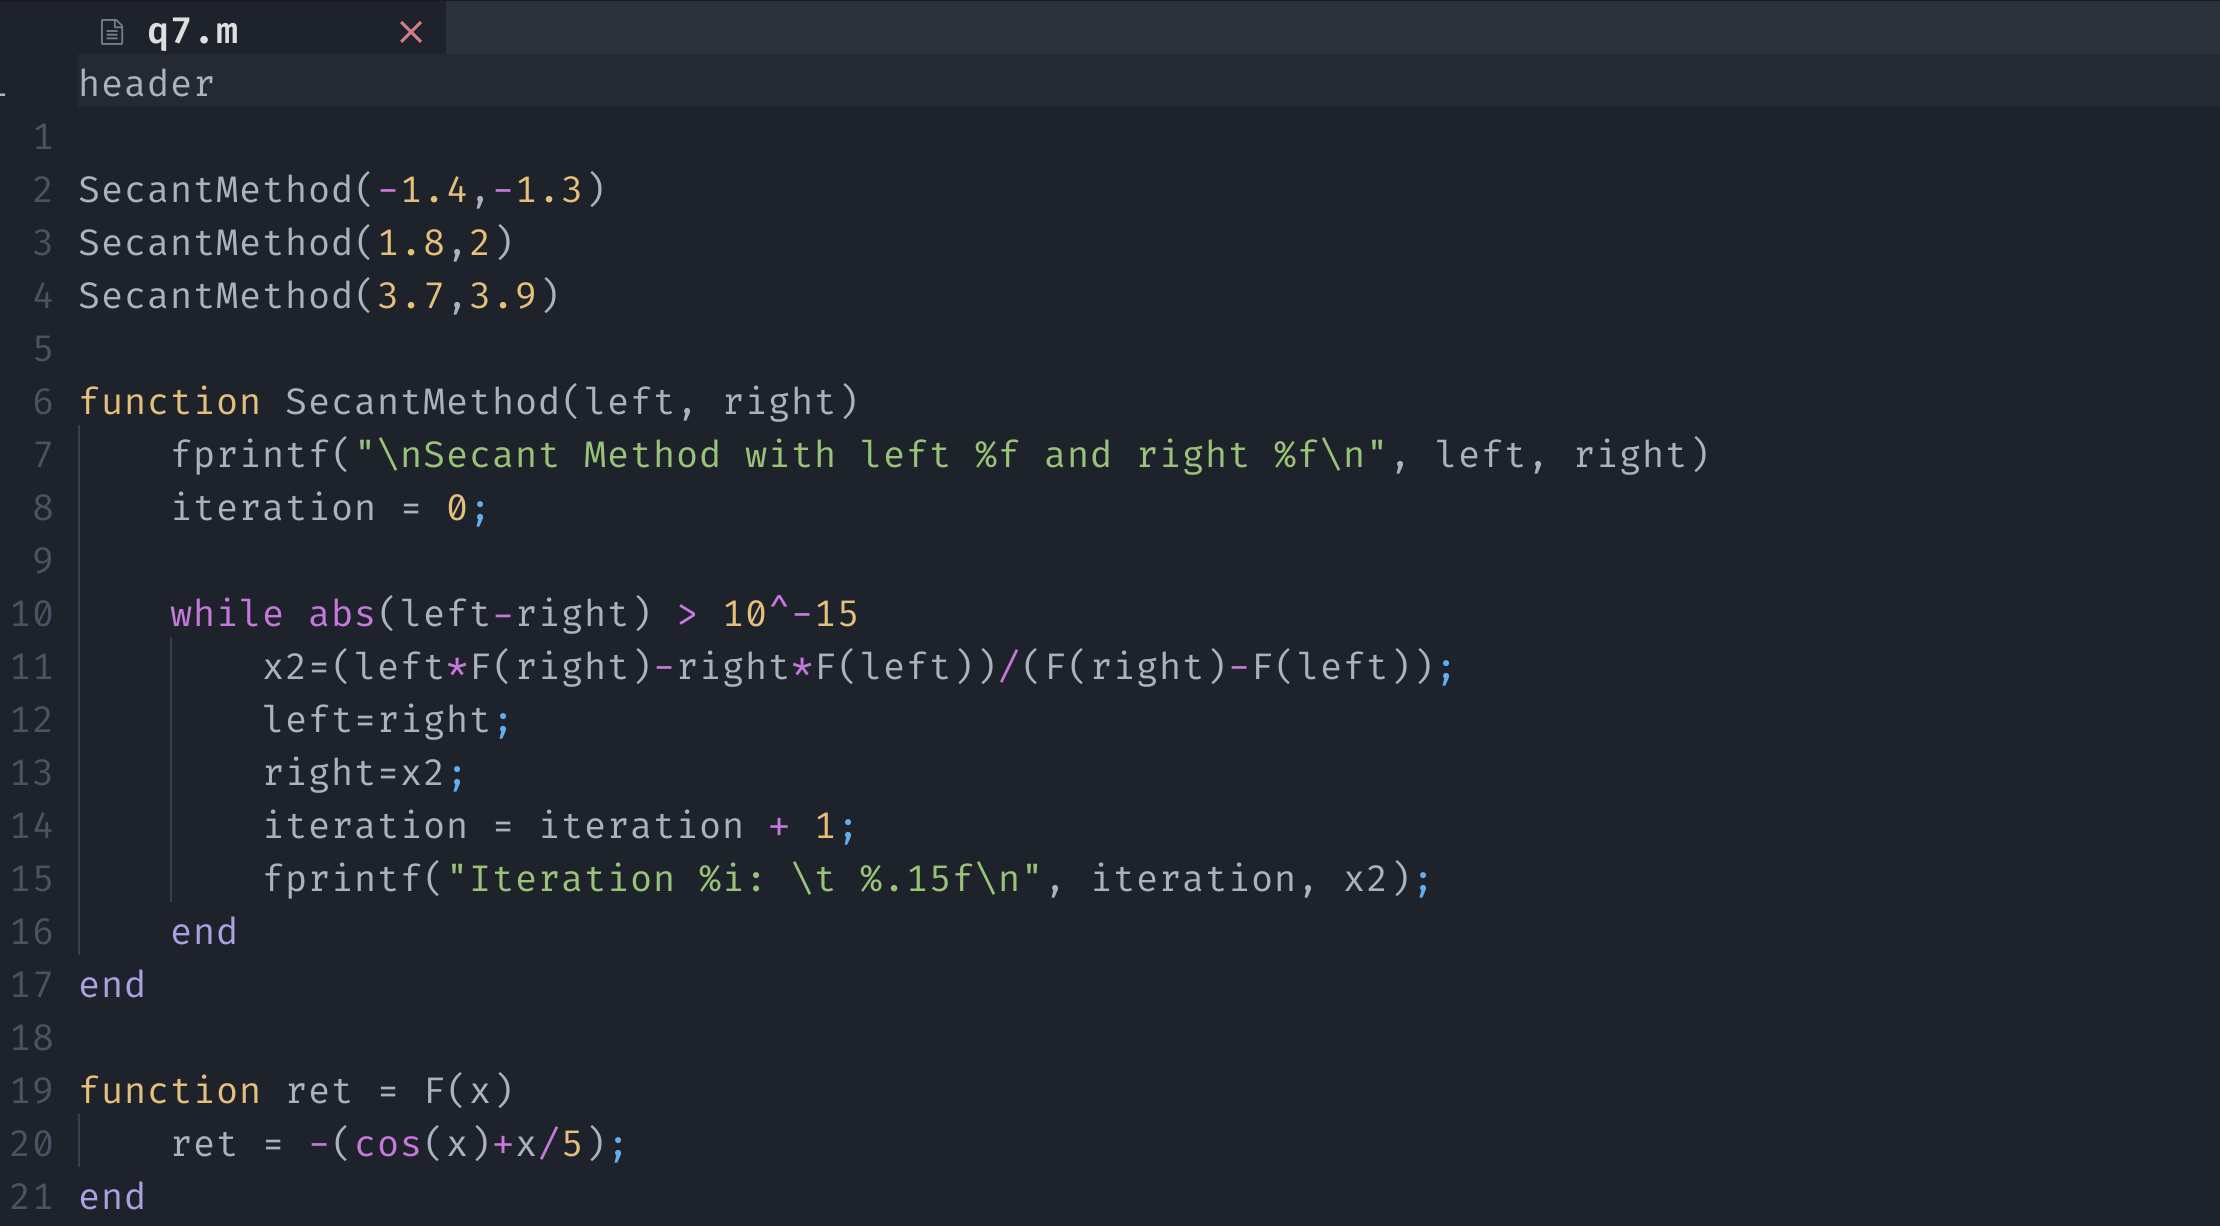
\includegraphics[width=0.8\textwidth]{imgs/q7_code.png}
	\caption{Code for question 7}
	\label{fig:q7_code}
\end{figure}

\begin{figure}[H]
	\centering
	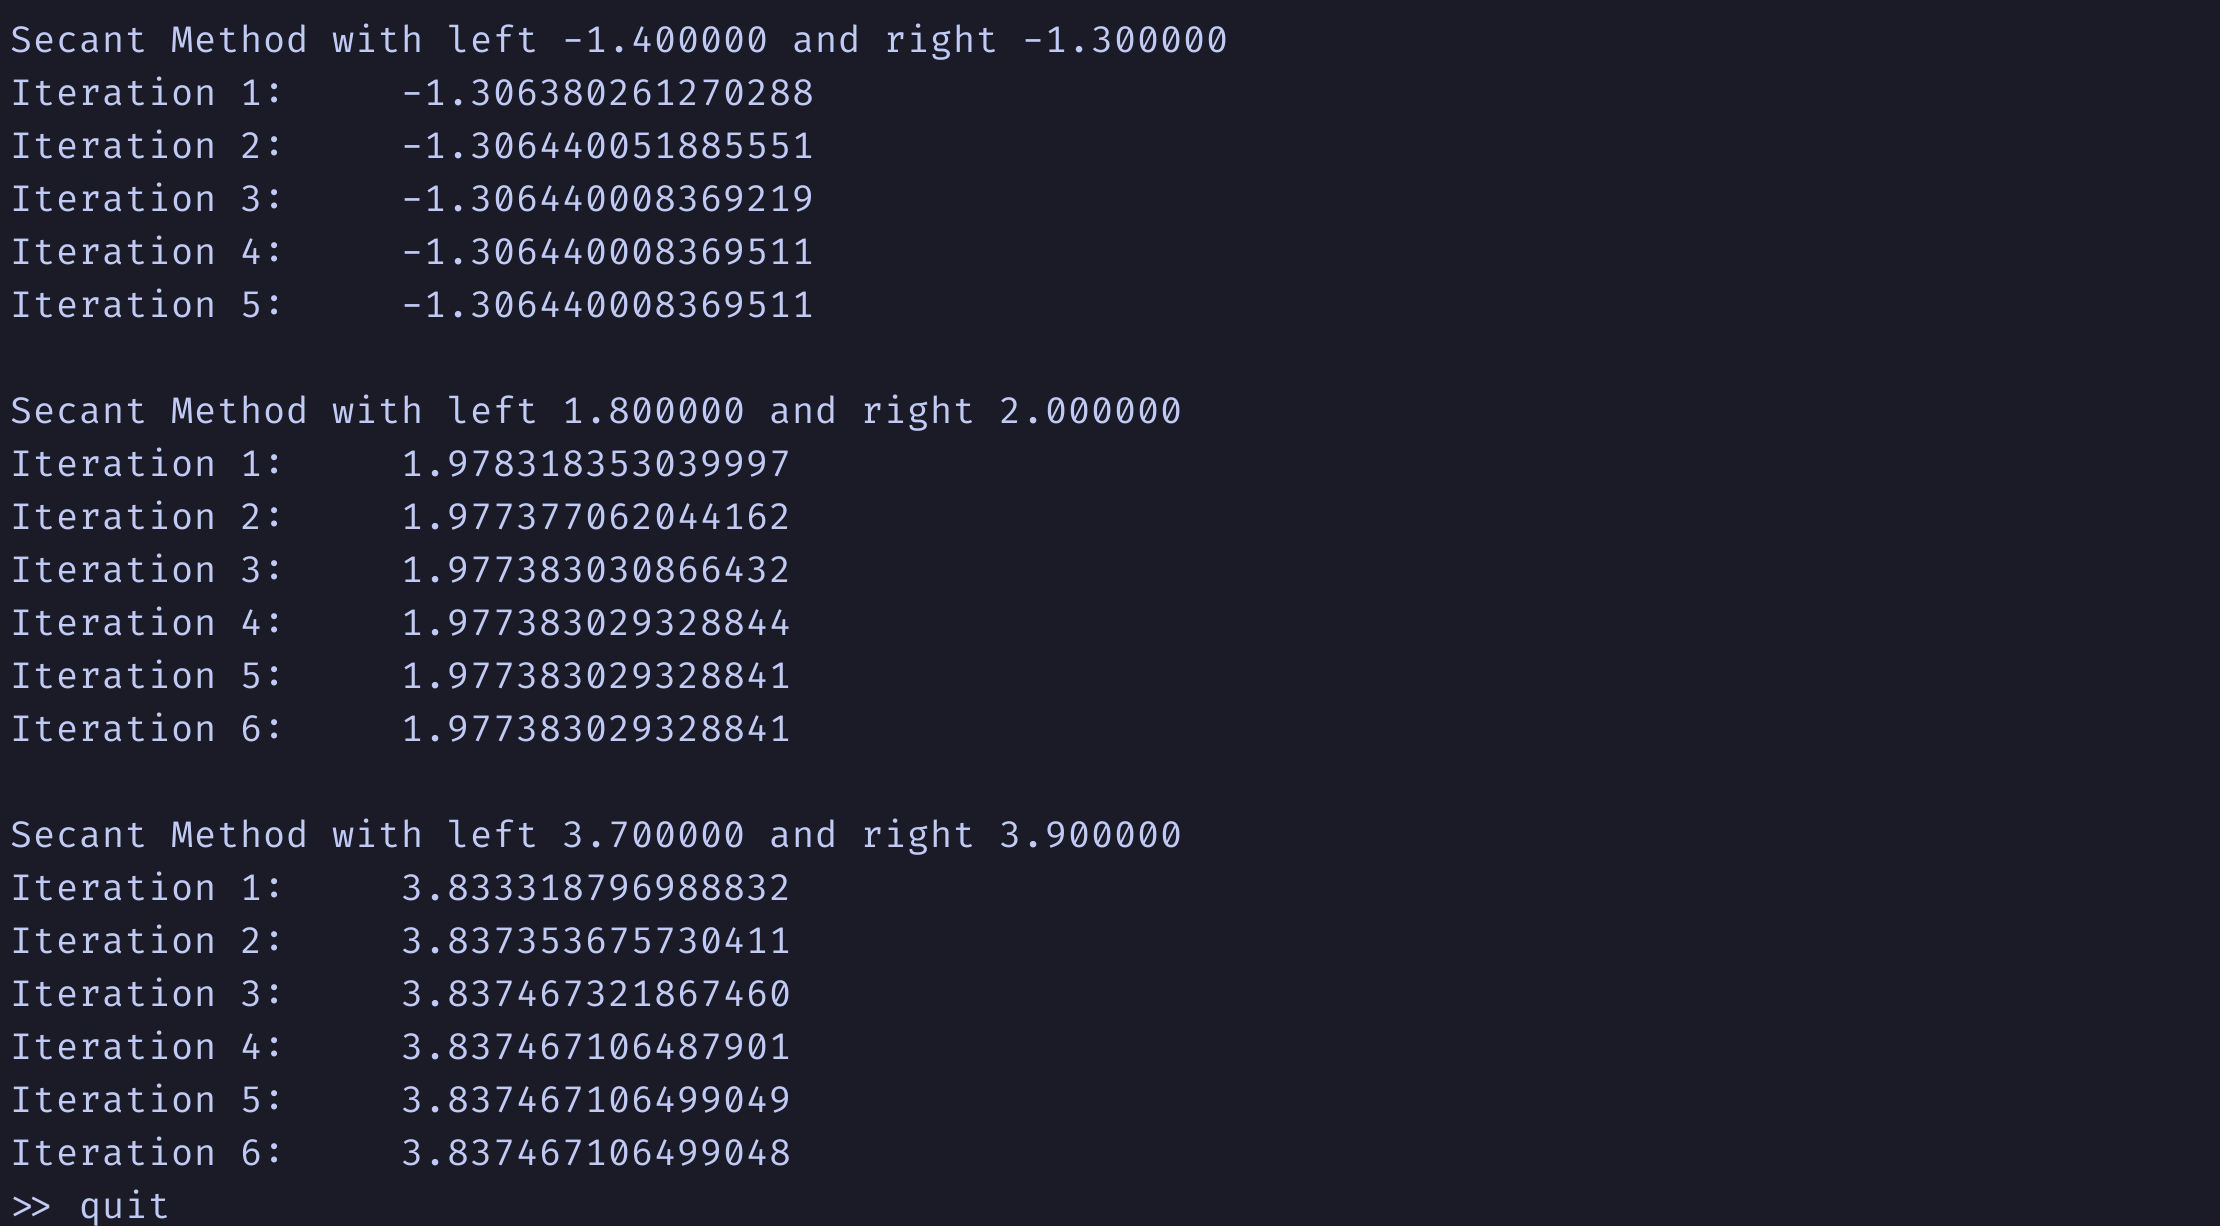
\includegraphics[width=0.8\textwidth]{imgs/q7_results.png}
	\caption{Results for question 7}
	\label{fig:q7_result}
\end{figure}

We can see that this method has slightly more iterations than the Newton Rhapson method had in the previous question. The notable differnce in uses of the functions is that the Secant method only needs the function itselft and not it's derivative but needs two initial guesses. 
Newton Rhapson on the other hand only requires one guess but needs the functions derivative. The Newton method generally converges a bit faster than the Secant method which is supported by our tests.


\newpage
\section{}

\begin{figure}[H]
	\centering
	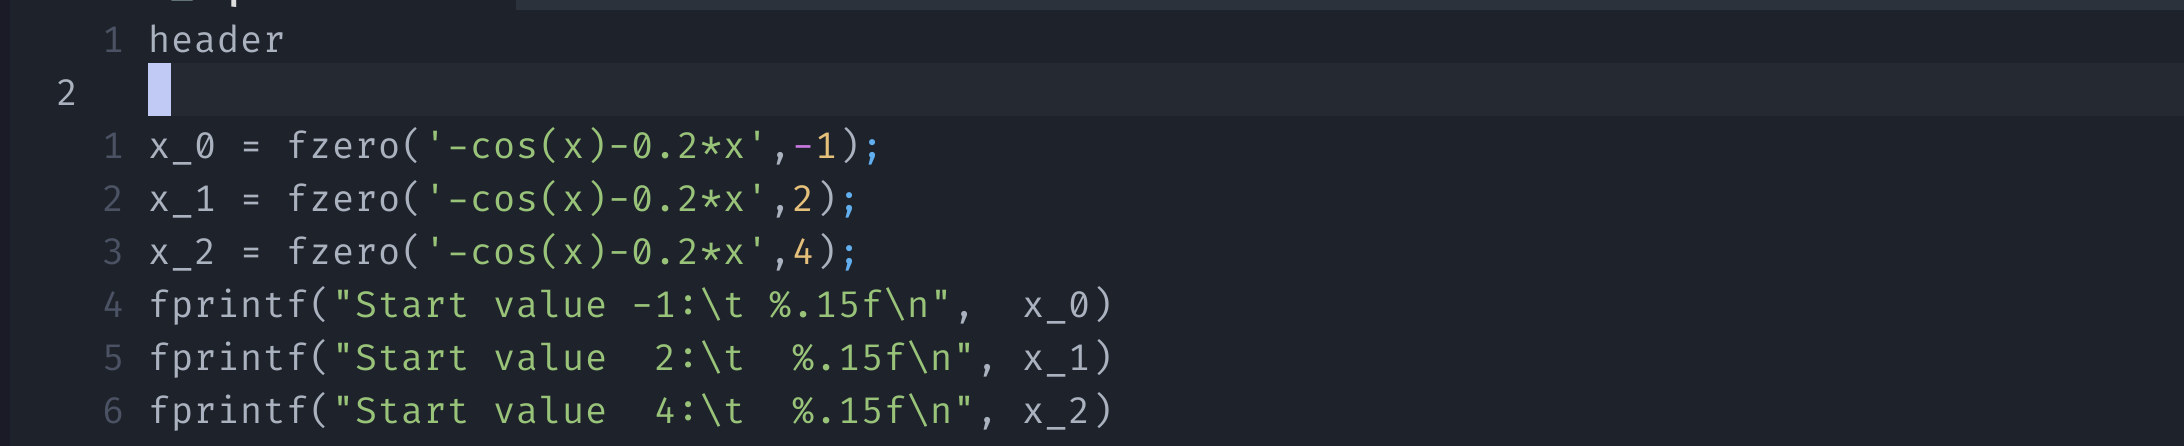
\includegraphics[width=0.8\textwidth]{imgs/q8_code.png}
	\caption{Code for question 8}
	\label{fig:q8_code}
\end{figure}

\begin{figure}[H]
	\centering
	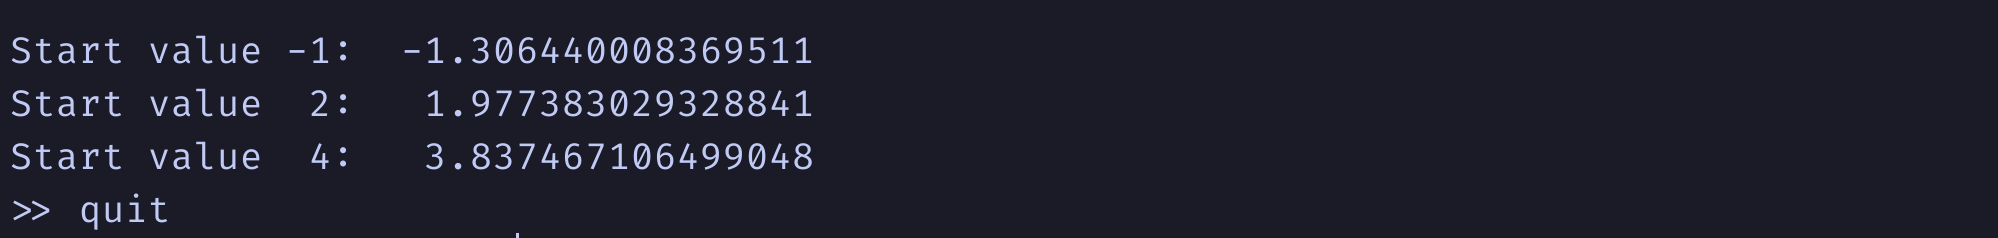
\includegraphics[width=0.8\textwidth]{imgs/q8_results.png}
	\caption{Results for question 8}
	\label{fig:q8_result}
\end{figure}






\end{document}
